%!TEX root = ../template.tex
%%%%%%%%%%%%%%%%%%%%%%%%%%%%%%%%%%%%%%%%%%%%%%%%%%%%%%%%%%%%%%%%%%%%
%% chapter2.tex
%% NOVA thesis document file
%%
%% Chapter with the template manual
%%%%%%%%%%%%%%%%%%%%%%%%%%%%%%%%%%%%%%%%%%%%%%%%%%%%%%%%%%%%%%%%%%%%
\chapter{Related Work}
\label{cha:users_manual}

% ================
% = Introduction =
% ================
Encryption of data stored in a computer is now more important than ever. Today we live in a world where almost every program we want to run or any application we want to use goes through a large number of different machines, therefore splitting our data through all. 

That is why it's needed to make sure all this information is unaccessible to potencial threats through encryption, regardless of which machine has the data. 

Although encrypting the stored data is a step forward towards the security of data, this is not enough. When one machine runs a program, the data needs to be decrypted and stored into RAM to be currectly executed, thus creating a potencial vulnerability. There is where Trusted Computing Environments come in.

We’ll look into more detail about existing technologies that approach this objective, and how they work or can work together as a way to grant confidentiality and integrity of data to the user.

(…) //TODO

In the summary, it’s expected to have a good notion of what has been developed in those areas to tackle this security concerns, as well as which of this thesis main points have already been addressed by previous work. (????)

\section{Trusted  Computing Environments} % (fold)
\label{sec:introduction}
We're currently in a period where we start to depend more and more on allowing other services to do our work for us. Technologies like cloud computing require users to trust these systems. Therefore it's needed something to grant some respectable level of security, as well as being able to grant trust to the user. That's were Trusted Computing Environments (TCE) come in handy.
A TCE is a concept that came to grant integrity and confidentiality to systems by forcing a certain machine to behave an expected way, and deny any unwanted access to the data while decrypted. This way, even if the system does not run in a trusted machine, it can be expected that it will execute as it should. 

TCEs also protect the system against components that should always be trusted, like the host OS or even system admins, due to the priviledges they've got. This prevention avoids this components to abuse these priviledges, and thus always guarantee the normal execution of the system. 

In the following sub-chapters we'll see how to achieve this properties, what components can be used to do it and also how each of them works.

\subsection{TPM – Trusted Platform Modules }

A Trusted Platform Module (TPM), proposed by the Trusted Computing Group (TCG), is a set of hardware and software technologies that aim to create trust in a local platform \cite{sgxCloudThesis}. It is identified by an Endorsment Key-pair (EK) which is unique for every TPM, and also a Storage Root Key (SRK) that is used to protect other keys and data in the TPM. 

As for the hardware, a TPM consists mainly on a chip, found usually in the motherboard of most machines nowadays, that provides and stores cryptographic keys that can be used to grant integrity and data confidentiality to the system, as well as persistent and volatile memory to store these keys. 

As said before, the main objective of a TPM is to create the idea of a trusted platform. This will be  provided by three main services: Encryption, Authenticated Boot and Attestation. The first one is used for pretty much every aspect related with security and privacy. The Authenticated boot consists in booting the OS in stages, as a way of keeping track of which code is trustable through the usage of Platform Configuration Registers (PCR), that store the trusted software hashes. As for the Attestation, we'll see in the next subsection.


\subsection{TPM – Enabled Software Attestation}


TPMs enable the use of Remote attestation, which is the capability of one system to determine if other system can be trusted to run a particular piece of software as expected or not.

This is made possible by having a trusted configuration of state as reference, provided by the PCRs defined in the boot sequence, followed by a remote system that proceeds to challenge the trusted platform (containing the TPM) with a nonce. Then the platform creates a message with the nonce received previously and the existing configuration and calculates an hash value for that message. With an Attestation Identity Key (AIK), the message is then signed and sent back to the remote system, which then proceeds to decrypt the message with the EK public part, that then compares the result with the hash of the nonce plus the configuration it had at the begining of the challenge. 

If the hashes match, the remote system can then identify the TPM platform as a trusted platform.

\subsection{HSM – Hardware Security Modules}

Hardware Security Modules (HSM) are physical components whose main function is to provide and store cryptographic keys used to encrypt/decrypt data inside a system. HSMs can also perform cryptographic operations (e.g. encryption, hashing, etc.) as well as authenticate through verification of digital signatures and accelerate SSL connections \cite{hsmThesis}.

This modules are used mainly in large environment systems (e.g. large distributed systems) where there are a lot of machines communicating with each other, therefore creating a more needed sense of security. The inclusion of this modules in these big systems is actually a good idea since HSMs can also help servers relieve the workload coming from cryptographic operations. However HSMs don't quite guarantee the idea of absolute security, but increment the cost of attacking the system.

Although HSMs grant some extra level of security to a system, there's some drawbacks. One of them is the cost, where to buy one HSM the price varies depending on the sophistication of the security, plus the cost of maintenance makes it even more expensive. Another disadvantage is the difficulty on updating the module. Let's say a weakness was found in a cryptographic algorithm, it's hard to update the software in an already functional HSM to eliminate that weakness \cite{hsmPaper}.

\subsection{Trusted Execution Environments}

A Trusted Execution Environment (TEE) is an abstraction provided by both software and hardware that guarantees isolated execution of specific programs from other programs running on the same machine \cite{guiBorgesThesis}, but also from the host OS, hypervisor or even system administrators, preventing them from leveraging their priviledges and thus take advantage of the system. A TEE also grants secured storage of sensitive data, as well as remote attestation to make sure a given program runs as expected on a remote TEE. 

For a user to communicate with his program running inside an isolated environment, a key-exchange between the TEE and the user takes place. This way it is ensured both integrity and confidentiality of data during further communications.

This TEE abstraction can be achieved either by using a virtual machine monitor or by running security critical software (from whole applications to little segments of code) under protection mechanisms provided by hardware \cite{pcopThesis}. 

In the next chapters we will be looking into more dept about this hardware protection providers, that are responsable to create this trusted environments in the systems nowadays.

\subsection{Intel SGX}

Intel Security Guard Extensions (SGX) are a set of instructions built in Intel CPUs, that allow programmers to create TEEs, called enclaves. Enclaves are isolation containers that create an isolated environment where sensitive code can be stored and executed inside, ensuring integrity and confidentiality to it. By doing so, it reduces the Trust Computing Base, in a way that most of the system software, apart from the enclaves itself, is considered not trusted.

Enclaves are mapped into private regions of memory, where only the CPU as access to, reducing the TCB to only the enclave and the CPU itself. Due to this restrictions, not even the most common system libraries can be accessed inside the enclave, since the OS is not trusted. 

A system that encorporates the SGX under it's architecture is divided in two components, a trusted being the enclave, and an untrusted being the rest of the system. The untrusted component requests the launch of the enclave, where the CPU then manages to allocate the enclave in a private region of memory, made available only to that particular enclave. This portion of memory is kept encrypted in volatile memory, being only decrypted by the CPU if the responsible enclave requests for it \cite{guiBorgesThesis}.

Altough isolation is the main objective of Intel SGX, it still allows a way for both  untrusted and trusted parties to communicate. This is made possible by the functions ECALL and OCALL. ECALLs are used for an untrusted component to call for trusted code in a secured way - the enclave copies the pointers to that specific code into a buffer, who is then made visible for the untrusted component, ensuring that the untrusted party can't know the real memory address inside the enclave. To communicate the other way arround the enclave calls for an OCALL, where the enclave is temporarily exited, executing then the unstrusted function needed. After that, the enclave is re-entered. This is mainly used by the enclave to access the network or to deal with I/O disk access.


\subsection{RISC-V enabled Sanctum}

Just like Intel SGX, the main objective of Sanctum is to offer strong isolation of software modules, altough following a different approach focused in avoiding unnecessary complexity, thus granting a simple security analysis.
To make this possible, Sanctum, which tipically runs in a RISC-V processor, combines minimal and minimally invasive hardware modifications with a trusted software security monitor that is receptive to analysis and does not perform cryptographic operations using keys. 

This minimality idea consists on reusing and slightly modifying existing well-understood mechanisms, while not modifiying CPU building blocks, only adding hardware to the interfaces between blocks, causing Sanctum to be adaptable to other processors in addition to RISC-V \cite{sanctumPaper}. 

Sanctum is a pratical approach that shows that a strong software isolation is achievable with a small set of minimally invasive hardware changes, causing reasonably low overhead. 
This approach provides strong security guarantees dealing with side-channel attacks, such as cache timing and passive address translation attacks.

\subsection{ARM Trust Zone}

ARM TrustZone are hardware security extentions offered by ARM application processors with the same finality as Intel SGX, create insolated environments where software execute in a trustable way. 

To accomplish this, ARM processors implement two virtual processors backed by hardware access control, where the software stack can switch between two states called secure world (SW) and normal world (NW). 
The first one has with higher priviledges than the second one, therefore it can access NWs copies of registers, but not the other way around. SW is also responsible of protecting running processes in the CPU, while providing secured access to peripherals. 
Each world acts like a runtime environment and has it's own set of resources. This resources can be partioned between the two worlds or just assigned to one of them, depending on the ARM chip.

For the context switch between worlds, ARM processors implement a secured mode called Secure Monitor, where there's a special register responsable of determine if the processor runs code in SW or NW. 

Most ARM processors also offer memory curtaining. This consists on the Secure Monitor allocating physical addresses of memory specifically to the SW, making this region of memory unaccessible to the rest of the system.

By default, the system boots always in SW so it can provision the runtime environment before any untrusted code start to run. It eventually transitions to NW where untrusted code can start to be executed. \cite{armTZPaper}


\subsection{AMD SEV}

AMD Secure Encrypted Virtualization (SEV) is the AMD approach to provide a TEE integrated with virtualization. It's a technology focused primarily on cloud computing environments, specifically in public infrastructure as a Service (IaaS), as its main goal is to reduce trust from higher priviledged parties (VMMs or OS), so that they can not influence the execution on the other "smaller" parties (VMs). 

To achieve this, AMD grants encryption of memory through a technology called Secure Memory Encryption (SEM), or through TransparentSEM (TSEM) if the system runs a legacy OS or hypervisor with no need for any software modifications.
After the data is encrypted, SEV integrates it with AMD virtualization architecture to support encrypted VMs. By doing this, every VM is now protected from his own hypervisor (VMM), unabling its access to the decrypted data. Although uncapable of accessing the VM, the VMM is still responsible of controlling each VM resources. \cite{amdPaper}

Thus, AMD provides confidentiality of data by removing trust from the VMM, and creates an isolated environment for the VM to run, where only the VM and the processor can be trusted. However it does not provide integrity of data, allowing replaying attacks to take place, and has a considerably large TCB, since the OS of each VM is trusted. \cite{amdSEVPaper}


\subsection{Discussion}

Write some comparison conclusions of why SGX and not the others.

//TODO


% section introduction (end)

% ====================
% = Folder Structure =
% ====================
\section{TEE/SGX Enabled Protection Against Untrusted OSes} % (fold)
\label{sec:folder_structure}

A lot of applications these days depend on sensitive data to operate and so protecting these data is very much taken into account while designing the application. 

One of the things we have to think about is the size of the TCB, and how to reduce it as much as possible without losing much of the operability of the system. Typically, the host OS is considered safe, trustworthy, although that is not always the case. A compromised OS can give complete access to this sensitive data in an application, regardless of how well designed it is, and that's why this is a major security problem to tackle in today's systems. 

In the following section will be discussed how to achieve security for this particular problem, how to remove the OS from our TCB without losing functionability of the system, preferably without any major drawbacks in the system's performance.

\subsection{Virtual Ghost}

Virtual Ghost was presented in 2014 \cite{virtGhostPaper} as an approach to provide application security against untrusted OSes without requiring higher privileges. 

To do so, it introduces the idea of ghost memory which is unaccessible to the OS to read or write, and provides the system with trusted services such as ghost memory management, key management, as well as encryption and signing services. 

Virtual Ghost therefore suggests a different design approach.
It uses compiler intrumentation to protect the system from external exploits of the OS, by sandboxing and using control-flow integrity and interposes a thin abstraction layer between the kernel and the hardware. Although this layer is similar to a hypervisor, it appears as a library of functions that the kernel code can call directly to interact with the hardware, thus avoiding the need of giving higher privileges than the OS itself. 

By using ghost memory and, as said before, preventing the OS from reading and writing ghost memory pages rather than allowing to access this regions of memory, Virtual Ghost makes the system safe from a direct threat from the OS.

Overhead for non-secure data is also prevented since, with that type of data, system calls made by the application don't need encryption or hashing.

Virtual Ghost gives the application flexibility on choosing the encryption and hashing algorithm, so that the system can obtain the desired tradeoff between performance and security.

It is an approach that offers protection from kernel malware, while ensuring comparable performance to TEEs, while adding a layer of protection against external attacks on the kernel itself.



\subsection{Flicker}

Flicker \cite{flickerPaper} is an infrastructure that provides secured isolated execution of sensitive code while trusting a small TCB, which significantly improves the security and reliability of the code Flicker executes. Although Flicker does not achieve the same level of protection from physical tampering as secure coprocessors do, it provides the same strong guarantees by using modern commodity hardware.

This isolation idea is guaranteed by trusting as few as 250 additional lines of code and, as a result, Flicker circumvents legacy software and eliminates reliance on their correctness, therefore reducing the TCB. Once the TCB has been precisely defined, it's possible for the system to achieve reliability and security.  

When Flicker starts, none of the software already executing can monitor or interfere with it's execution. Also, all traces of it's execution can be eliminated before non-Flicker execution resumes.

It also provides fine-grained attestation of the code executed to an external party, where the party using Flicker does not leak any information about the state of the system software. 

To achieve these properties, Flicker needs hardware that support late launch and attestation, such as AMD and Intel commodity processors, and it's still capable of guarantee them even if the BIOS and OS have become malicious to the system.

\subsection{MUSHI}

MUSHI, or MUltiple level Security cloud with strong Hardware level Isolation, is a framework that provides hardware level isolation and protection to individual guest VMs executing in a cloud infrastructure. It guarantees confidentiality and integrity of a VM even during malicious attacks from both inside and outside the cloud environment.

MUSHI is mainly designed to deal with multi-level security (MLS) \cite{mlsMIT} systems, therefore MUSHI's main goal is to provide a trusted isolated environment for VM execution. To achieve this, VMs should be instantiated securely and should remain that way throughout their life cycle. With that in mind, MUSHI guarantees the following properties

\begin{itemize}
	\item Trusted Execution - upon starting a VM, the integrity of both kernel and user image, as well as MUSHI itself, should be attested to the user, thus defining a trusted initial state

	\item Isolation - VMs running on the same machine should be isolated. As a result, both confidentiality and integrity will be provided to the user VM during execution. However it does not prevent side channel attacks
	
	\item User Image Confidentiality - MUSHI provides user image encryption with a key provided by the user itself
	
\end{itemize}

MUSHI depends on a very small TCB, including only the hardware, hardware virtualization, BIOS and System Management Mode. It can be implemented using modern commodity hardware containing SMM memory (SMRAM), necessary for the isolation between the host and VM. For remote attestation of VM images, it's done used a TPM. \cite{mushiPaper}


\subsection{SeCage}

SeCage \cite{SeCagePaper} is an approach that aims to protect user-defined secrets from application potential threats and malicious OS through hardware virtualization, thus isolating sensitive code and critical secrets while denying hypervisor intervention during runtime.
It's designed to deal with a strong adversary model, assuming that both application and OS can be compromised, while suporting large-scale software, which usually means a big attack surface.

SeCage devides the system in compartments, where secret compartments have all the functions with permissions to access and manipulate those secrets, and a main compartment is resposible to handle the rest of the code.

The main goals of SeCage are to assure confidentiality of user secrets (e.g., cryptographic keys) and to be a pratical approach with small overheads for large software systems. To achieve this, it ensures

\begin{itemize}
	\item Hybrid analysis of secrets - provides a mechanism that prevents secrets from being disclosed during runtime, while not affecting their normal usage. For it, SeCage combines static and dynamic analysis. The first one is used to discover potencial functions related to the secrets, while the second one complements the first one, being more precise than the first one. With this, SeCage defines secret compartments, containing a set of secrets and their most common functions. This ensures that only the functions inside a compartment can access that set of secrets.  
	\item Hypervisor protection - isolate each compartment in a completely isolated address space through hardware virtualization, making them unaccessible to the Hypervisor. Only if a function outside a compartment tries to access a secret without permission, it's the Hypervisor job to handle that violation.
	\item Separating control and data plane - since each compartment needs to communicate with each other, there will eventually be contact with the hypervisor. Therefore, instead of frequent VM exits which cause high overheads, SeCage minimazes hypervisor intervention by only require it to define policies on whether two compartments can communicate (control plane) for as long as they conform to those policies (data plane)
	
\end{itemize}

SeCage was shown useful protecting large-scale system software from HeartBleed attacks, kernel memory disclosure and rootkit memory scanning, without adding any significant performance overhead to the application.


\subsection{InkTag}

InkTag \cite{inkTagPaper} is a virtualization-based architecture that protects trusted applications from an untrusted OS, allowing trusted applications to securely use untrusted OS services. InkTag admits trust in the hypervisor, which is responsible to protect the application code, data, and control flow from the OS, allowing applications to execute in isolation, in a high-assurance process (HAP). 
Trusted applications can securely and privately share data without interference from the OS or other applications. Each secure application communicates directly with the InkTag hypervisor via hypercalls to detect OS misbehavior.

It introduces a concept called paraverification, which is a technique that simplifies the hypervisor by forcing the untrusted OS to participate in its own verification. As a result, the OS notifies the hypervisor when there is any update to be made to the state, which the hypervisor then checks for correctness.
InkTag also ensures virtualization through hardware, which is used to grant isolation, as well as separate secure from insecure data.
Access control policies can be specified by each trusted applications to access their secure files, with privacy and integrity of them managed by InkTag through encryption and hashing. 
 
Other important aspect of InkTag is recoverability. InkTag is capable of ensuring crash consistency between file data and metadata. Metadata, which consists in hashed data, is fundamental to guarantee integrity of data therefore, with this consistency granted, InkTag hypervisor can protect the integrity of files even if the system crashes. If for some reason some data is inconsistent, the application must discard it.





\subsection{Sego}

Sego \cite{segoPaper} is a hypervisor-based system that gives strong privacy and integrity guarantees to trusted applications, even when the guest OS is compromised or hostile, by removing the trust from the OS. Sego verifies OS services, like the file system, instead of replacing them.

To protect the application from the untrusted OS, Sego relies on a trusted hypervisor and assumes that hardware always executes hypervisor code correctly.
It uses paraverification, where the guest OS communicates its actions and intent to the hypervisor, therefore making this verification of the untrusted OS behavior more efficient and easy.

\begin{figure}[htbp]
	\centering
	{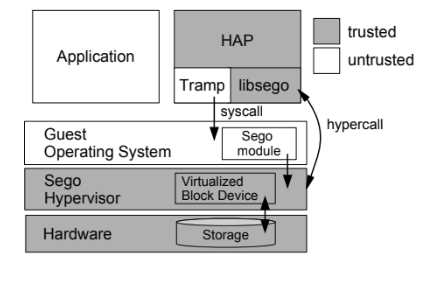
\includegraphics[width=0.5\linewidth]{sego_architecture}}%
	\caption{Sego Architecture Overview}
\end{figure}


Sego executes trusted code in a HAP. After booting the OS, the hypervisor starts the HAP in a way that the HAP itself can verify its own initial code and data, similar to a TPM. Once running, the hypervisor ensures that HAP's registers and trusted address space are isolated from the OS. 
Everytime the HAP wants to perform a system call, it must inform the hypervisor of its intent, so that the hypervisor can verify OS activity. HAPs use a small library called libsego as a way to handle system calls and get Sego services without having to change their code. 
Each HAP also contains an untrusted trampoline code, that uses to interact with the OS. This is used as a way to protect HAP control-flow, since it uses this trampoline as the issuer for the system calls, therefore never compromising the HAP itself.



Context switches are handled by the hypervisor, hiding any information about the HAP from the OS.

Sego does not guarantee OS availability. A compromised OS can simply shut down or refuse to schedule processes. However this is easily detected.




\subsection{Other approaches}

There are also other approaches that tackle the same problem of trusting the OS, making it impossible for the execution of an  application to be compromised by a malicious OS, such as 

\begin{itemize}
	\item Hardware-assisted Data-Flow Isolation (HDFI) \cite{hdmiPaper} - data isolation mechanism running on top of RISC-V that uses machine instructions and hardware to enforce isolation, by virtually extending each memory unit with an additional tag that is defined by data-flow. It grants stack protection, standard library enhancement, kernel data protection, virtual function table protection, code pointer protection and information leak prevention. It's easy to use and imposes low performance overhead, while improving security.
	
	\item Secure Channel between Rich Execution Environment and Trusted Execution Environment (SeCReT) \cite{secretPaper} - it is a framework that is focused in securing the communications between the Rich Execution Environments (REE) and the TEE built in ARM TrustZone, to add to the idea of isolation from the OS. It enables legitimate processes to use a session key in the REE, which is regarded as unsafe. To protect the key, SeCReT verifies the code's integrity and control-flow of the process every time a switch between user mode and kernel mode takes place. SeCReT's key-protection mechanism is only activated during the runtime of the process that has permission to access TrustZone, so it minimizes the performance overhead.
	




\subsection{Discussion}

Another conclusion about the differences of the approaches. 
 
//TODO







% section folder_structure (end)

% ===================
% = Package options =
% ===================
\section{SGX-Frameworks and Application Support} % (fold)
\label{sec:package_options}
\subsection{VC3 protection for MapReduce Jobs}
\subsection{Protected Zookeeper}
\subsection{Ryoan Sandboxing}
\subsection{Opaque}
\subsection{Graphene-SGX}
\subsection{Network services protection approaches}
\subsection{Application-level protection approaches}
\subsection{Discussion}


The \novathesis\ class can be customized with the options listed below.

\newcommand{\classoption}[3]{\textbf{#1=OPT}\qquad #2\\\qquad\emph{#3}\\}

\noindent
\begin{ctabular}{@{}p{\linewidth}@{}}
  \toprule
  \classoption{docdegree}%
    {phd(*), phdplan, phdprop, msc, mscplan, bsc}%
    {The type of the document: PhD Thesis (default), PhD Plan, PhD Proposal, MSc Disseration, MSc Plan, BSc Report}
    \midrule
  \classoption{school}%
		{nova/fct(*), nova/fcsh, nova/ims, ul/ist, ul/fc}%
    {The name of the school. This option changes the typesetting of the cover and some School specific formating, like margins, fonts, paragraph spacing and indentation, etc…}
    \midrule
  \classoption{lang}%
    {en(*), pt}%
    {The main language for the document.  Currently only Portuguese and English are supported.  Other languages are expected to be support in forthcoming versions.}
    \midrule
  \classoption{fontstyle}%
    {bookman, charter, fourier, kpfonts(*), mathpazo1, mathpazo2, newcent}%
    {The font set to be used in the document.  Please note that a font set include definitions for the main text, headings, maths, etc.}
    \midrule
  \classoption{chapstyle}%
    {bianchi, bluebox, brotherton, dash, default, elegant(*), ell, ger, hansen, ist, jenor, lyhne, madsen, pedersen, veelo, vz14, vz34, vz43}%
    {The chapter style, i.e., the look of the chapter beginning.}
    \midrule
  \classoption{converlang}%
    {en, pt(*)}%
    {The language to be used when typesetting the cover page.}
    \midrule
  \classoption{otherlistsat}%
    {front(*), back}%
    {Where to put the other lists besides the table of contents. The default is (\texttt{front}) before the main text.  But some scientific areas prefer them at the end of the document (\texttt{back}), just before the Appendixes.}
    \midrule
  \classoption{aftercover}%
    {true, false(*)}%
    {Include or don't include the contents of the “\texttt{aftercover}” file. The default is for this file to be ignored (if if it exists).}
    \midrule
  \classoption{linkscolor}%
    {darkblue(*), black}%
    {The color for all the hyperlinks in the PDF file.  The “\texttt{media=paper}” option (see below) will override this option to “\texttt{black}”}
    \midrule
  \classoption{spine}%
    {true, false(*)}%
    {Generate the book spine and the last page in the PDF.}
    \midrule
  \classoption{biblatex}%
    {OPT=\{list of options for \texttt{biblatex}\}}%
    {Customize \texttt{biblatex}, the bibliography management system used in this class. Probably you will want to change the value of the \texttt{biblatex} “\texttt{style}” option. For other customizations of \texttt{biblatex} check its manual.}
    \midrule
  \classoption{memoir}%
    {OPT=\{list of options for \texttt{memoir}\}}%
    {Customize the base class \texttt{memoir}. The \texttt{memoir} manual should be the first document to be consulted when looking for “\textbf{how can I do this?}” You may wnat to change the base font size from 11pt to a smaller (10pt) or larger (12pt) size.  Also, remember to change the “\texttt{draft}” to final when your document is finished.}
    \midrule
  \classoption{media}%
    {screen(*), paper}%
    {Behavior to be customized in the school options/configuration. Expected definitions for screen are: left and right margins are equal and use colored links. Expected definitions for paper are: left and right margins are different and use black links.}
    \bottomrule
\end{ctabular}

\section{Related work analysis and rational} % (fold)
\label{sec:additional_considerations}

In this section we will provide some additional considerations about some of the customizations available as class options.



